\documentclass[hidelinks,12pt]{article}
% \usepackage{../Estilos/ColoresLatex}
\usepackage[left=0.25cm,top=1cm,right=0.25cm,bottom=1cm]{geometry}
%\usepackage[landscape]{geometry}
\textwidth = 20cm
\hoffset = -1cm
\usepackage[utf8]{inputenc}
\usepackage[spanish,es-tabla, es-lcroman]{babel}
\usepackage[autostyle,spanish=mexican]{csquotes}
\usepackage[tbtags]{amsmath}
\usepackage{nccmath}
\usepackage{amsthm}
\usepackage{amssymb}
\usepackage{mathrsfs}
\usepackage{graphicx}
\usepackage{subfig}
\usepackage{caption}
%\usepackage{subcaption}
\usepackage{standalone}
\graphicspath{{Imagenes/}{../Imagenes/}}
\usepackage[outdir=./Imagenes/]{epstopdf}
\usepackage{siunitx}
\usepackage{physics}
\AtBeginDocument{\RenewCommandCopy\qty\SI}
\ExplSyntaxOn
\msg_redirect_name:nnn { siunitx } { physics-pkg } { none }
\ExplSyntaxOff
\usepackage{color}
\usepackage{float}
\usepackage{hyperref}
\usepackage{multicol}
\usepackage{multirow}
%\usepackage{milista}
\usepackage{anyfontsize}
\usepackage{anysize}
%\usepackage{enumerate}
\usepackage[shortlabels]{enumitem}
\usepackage{capt-of}
\usepackage{bm}
\usepackage{mdframed}
\usepackage{relsize}
\usepackage{placeins}
\usepackage{empheq}
\usepackage{cancel}
\usepackage{pdfpages}
\usepackage{wrapfig}
\usepackage[flushleft]{threeparttable}
\usepackage{makecell}
\usepackage{fancyhdr}
\usepackage{tikz}
\usepackage{bigints}
\usepackage{tcolorbox}
\tcbuselibrary{breakable}
\usepackage{scalerel}
\usepackage{pgfplots}
\usepackage{pdflscape}
\usepackage{enumitem}
\pgfplotsset{compat=1.16}
\spanishdecimal{.}
\renewcommand{\baselinestretch}{1.5}
\def\scaleint#1{\vcenter{\hbox{\scaleto[3ex]{\displaystyle\int}{#1}}}}
\def\scaleoint#1{\vcenter{\hbox{\scaleto[3ex]{\displaystyle\oint}{#1}}}}
\def\scaleiint#1{\vcenter{\hbox{\scaleto[3ex]{\displaystyle\iint}{#1}}}}
\def\scaleiiint#1{\vcenter{\hbox{\scaleto[3ex]{\displaystyle\iiint}{#1}}}}
\def\bs{\mkern-12mu}

\newcommand{\Cancel}[2][black]{{\color{#1}\cancel{\color{black}#2}}}

% \newcommand{\qed}{\tag*{$\blacksquare$}}
\renewcommand{\qed}{\hfill\blacksquare}

\usepackage{titling}


\title{Lista de ejercicios del Tema 1 \\[0.3em]  \large{Matemáticas Avanzadas de la Física}\vspace{-3ex}}
\author{M. en C. Gustavo Contreras Mayén}
\date{ }

\setlength{\droptitle}{-3cm}

\begin{document}

\vspace{-6cm}
\maketitle

\fontsize{14}{14}\selectfont

\noindent
\textbf{Nota importante:} Considera que conforme se vayan presentando los ejercicios en clase, se actualizará el documento para que tengas los enunciados y vayas resolviendo cada ejercicio de manera oportuna.
\\[0.75em]
\noindent
\textbf{Indicaciones: } Se te pide gentilmente que resuelvas de manera detallada, clara y ordenada los siguientes ejercicios, el puntaje que otorga cada enunciado es de \textbf{1 punto}. En caso de que requieras apoyarte en alguna propiedad, si fue vista en clase, solo indícalo, pero si esa propiedad aunque esté relacionada al ejercicio y no se haya mencionado en clase, habrá que demostrarla debidamente.

\begin{enumerate}
\item Considera la transformación de coordenadas:
\begin{align*}
x &= 2 \, u \, v \\[0.5em]
y &= u^{2} + v^{2} \\[0.5em]
z &= w
\end{align*}
Demuestra que el nuevo sistema de coordenadas \textbf{es no ortogonal}.
\item Considera la transformación de coordenadas:
\begin{align*}
x &= 2 \, u \, v \\[0.5em]
y &= u^{2} - v^{2} \\[0.5em]
z &= w
\end{align*}
Demuestra que el nuevo sistema de coordenadas \textbf{es ortogonal}.
\item Escribe en coordenadas esféricas $(r, \theta, \phi)$ el siguiente vector:
\begin{align*}
\vb{A} = x \, y \, \vu{i} - x \, \vu{j} + 3 \, x \, \vu{k}
\end{align*}
adicionalmente expresa $A_{r}, A_{\theta}, A_{\phi}$ en términos de $r, \theta, \phi$.
\item La velocidad y la aceleración se definen en la forma vectorial como:
\begin{align*}
\vb{v} = \dv{\vb{r}}{t} = \dot{\vb{r}} \hspace{1cm} \vb{a} = \dot{\vb{v}} = \ddot{\vb{r}}
\end{align*}
Calcula para el sistema coordenado esférico:
\begin{enumerate}
\item $\dot{\vu{e}}_{r}$, $\dot{\vu{e}}_{\theta}$, $\dot{\vu{e}}_{\varphi}$ 
\item La velocidad: $\vb{v}$
\item La aceleración: $\vb{a}$
\end{enumerate}
\item Demuestra que $\grad{\left( \phi \psi \right)} = \phi \, \grad{\psi} + \psi \, \grad{\phi}$
\item Si $f = f(r)$ con $r = \sqrt{x^{2} + y^{2}+ z^{2}}$, demuestra que
\begin{align*}
\nabla{f(r)} = \vu{r} \, \dv{f(r)}{r}
\end{align*}
\item Demuestra que el campo eléctrico de una carga puntal
\begin{align*}
\vb{E} = \dfrac{q \, \vu{r}}{4 \, \pi \epsilon_{0} \, r^{2}}
\end{align*}
cumple $\div{\vb{E}} = 0$, para $r \neq 0$.
\item El campo electrostático de un dipolo eléctrico $\vb{p} = p_{0} \, \vu{e}_{z}$ es:
\begin{align*}
\vb{E} = \dfrac{p_{0} (2 \, \vb{e}_{r} \, \cos \theta + \vu{e}_{\theta} \, \sin \theta)}{r^{3}}
\end{align*}
Demuestra que:
\begin{enumerate}
\item $\curl{\vb{E}} = 0$
\item para $r \neq 0$, se tiene $\div{\vb{E}} = 0$
\end{enumerate}
\item Usando coordenadas curvilíneas demuestra que:
\begin{align*}
\laplacian{(\phi \, \psi)} = \phi \, \laplacian{\psi} + \psi \, \laplacian{\phi} + 2 \, \grad{\phi} \vdot \grad{\psi}
\end{align*}
\item Para el sistema de coordenadas esferoidales prolatas $(\xi, \eta, \phi)$, cuyas reglas de transformación son:
\begin{align*}
x &= a \: \sinh \xi \: \sin \eta \: \cos \phi\\
y &= a \: \sinh \xi \: \sin \eta \: \sin \phi\\
z &= a \: \cosh \xi \: \cos \eta
\end{align*}
\begin{enumerate}
\item Describe las superficies coordenadas del sistema.
\item Calcula de manera explícita los factores de escala $(h_{\xi}, h_{\eta}, h_{\phi})$.
\item Describe los vectores unitarios $(\vu{e}_{\xi}, \vu{e}_{\eta}, \vu{e}_{\phi})$
\item Recupera los operadores diferenciales: gradiente, divergencia, rotacional y Laplaciano en este sistema coordenado.
\end{enumerate}
\item En una distribución tipo Maxwell la fracción de partículas moviéndose con velocidad $v$ y $v +\dd{v}$ es
\begin{align*}
\dfrac{\dd{N}}{N} = 4 \, \pi \left( \dfrac{m}{2 \, \pi \, k \, T} \right)^{3/2} \: \exp \left( - \dfrac{m \, v^{2}}{2 \, k \, T} \right) \: v^{2} \dd{v}
\end{align*}
donde $N$ es el número total de partículas. 
\par
El promedio o valor esperado de $v^{n}$ se define como $\displaystyle \expval{v^{n}} = N^{-1} \int v^{n} \dd{N}$.
\par
Demostrar que:
\begin{align*}
\expval{v^{n}} = \left( \dfrac{2 \, k \, T}{m} \right)^{n/2} \dfrac{\left( \dfrac{n + 1}{2} \right) !} { \left( \dfrac{1}{2} \right) !}
\end{align*}
\item Se muestra en la figura (\ref{fig:figura_cicloide}) parte de una cicloide cuyas ecuaciones paramétricas son
\begin{align*}
x &= a (\theta + \sin \theta) \\[0.5em]
y &= a (1 - \cos \theta)
\end{align*}
\begin{figure}
    \centering
    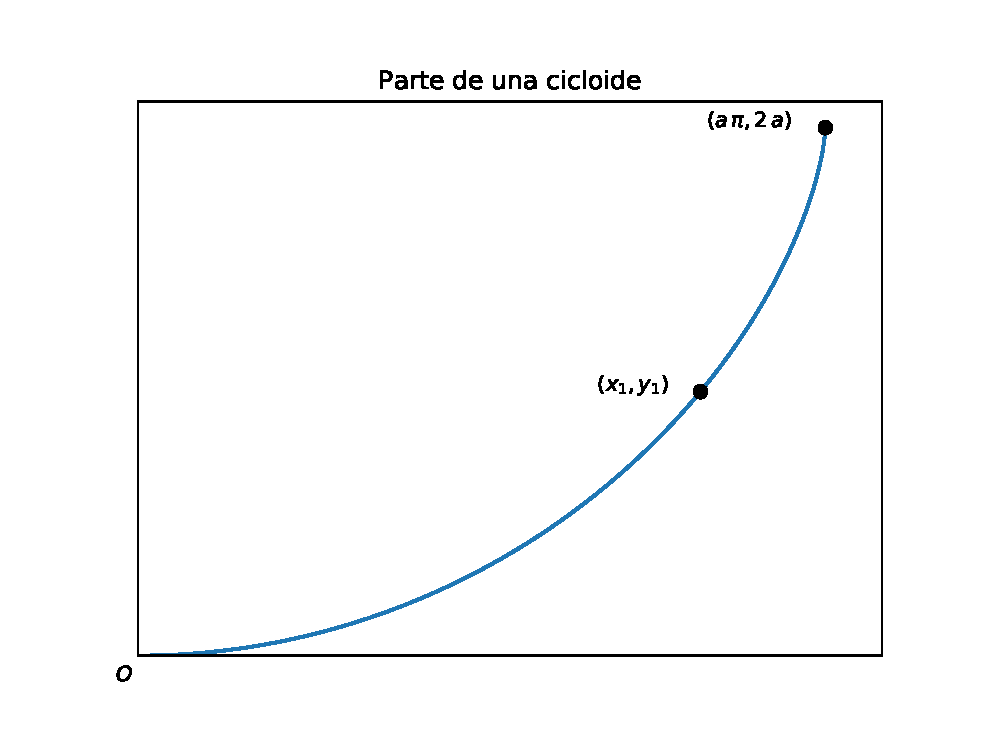
\includegraphics[width=0.75\textwidth]{Imagenes/plot_cicloide.eps}
    \caption{Una partícula deslizándose sobre una cicloide.}
    \label{fig:figura_cicloide}
\end{figure}
Demuestra que el tiempo que tarda una partícula para deslizarse sin fricción a lo largo de la curva desde el punto $(x_{1}, y_{1})$ hasta el origen, está dado por
\begin{align*}
t = \sqrt{\dfrac{a}{g}} \, \int_{0}^{y_{1}} \dfrac{\dd{y}}{\sqrt{y \, (y_{1}- y)}}
\end{align*}
Sugerencia: Demuestra que la longitud del elemento de arco es
\begin{align*}
\dd{s} = \sqrt{\dfrac{2 \, a}{y}} \dd{y}
\end{align*}
Evalúa la integral para demostrar que el tiempo es independiente de la posición inicial $y_{1}$.
\end{enumerate}

\end{document}